%%%%%%%%%%%%%%%%%%%%%%%%%%%%%%%%%%%%%%%%%%%%%%%%%%%%%%%%%%%%%%%%%%%%%%%%%
% Angaben zur Person
%%%%%%%%%%%%%%%%%%%%%%%%%%%%%%%%%%%%%%%%%%%%%%%%%%%%%%%%%%%%%%%%%%%%%%%%%
\newcommand{\name}{Dennis Pidun}
\newcommand{\matr}{??????}
\newcommand{\email}{pidund@uni-hildesheim.de}
\newcommand{\studgang}{Angewandte Informatik (B.Sc.)}
\newcommand{\thema}{Safety Engineering in AGI}
\newcommand{\keywords}{}
\newcommand{\betreuer}{Dr. Pascal Reuß}

%%%%%%%%%%%%%%%%%%%%%%%%%%%%%%%%%%%%%%%%%%%%%%%%%%%%%%%%%%%%%%%%%%%%%%%%%
% Angaben zum Seminar
%%%%%%%%%%%%%%%%%%%%%%%%%%%%%%%%%%%%%%%%%%%%%%%%%%%%%%%%%%%%%%%%%%%%%%%%%
\newcommand{\semester}{Wintersemester 2019/2020}
\newcommand{\vtyp}{Seminar}
\newcommand{\veranstaltung}{IIS Seminar}
\newcommand{\prof}{Prof. Dr. Klaus-Dieter Althoff}
\newcommand{\lehrstuhl}{Institut für Informatik\\Bereich Intelligente Informationssysteme}

%%%%%%%%%%%%%%%%%%%%%%%%%%%%%%%%%%%%%%%%%%%%%%%%%%%%%%%%%%%
%% Diese Datei sollten Sie nicht anpassen, sie definiert %%
%% ein Dokument der Form, in der wir es erwarten.        %%
%%%%%%%%%%%%%%%%%%%%%%%%%%%%%%%%%%%%%%%%%%%%%%%%%%%%%%%%%%%

%Schriftgr��e, ein- oder zweiseitig, Papierformat, Dokumententyp
\documentclass[12pt,oneside,a4paper]{scrartcl}

\usepackage[latin1]{inputenc}
%Seitenr�nder
\usepackage[left=2.5cm,right=2.5cm,top=2.5cm,bottom=2cm]{geometry}

%NDR und Umlaute
\usepackage{ngerman}
\usepackage[latin1]{inputenc}

%Kopf- und Fu�zeile
\usepackage{fancyhdr}
\pagestyle{fancy}
\fancyhf{}

%Kopfzeile links bzw. innen
\fancyhead[L]{\name}

%Kopfzeile mittig
\fancyhead[C]{\thepage}

%Kopfzeile rechts bzw. au�en
\fancyhead[R]{\thema}

%Linie oben
\renewcommand{\headrulewidth}{0.5pt}

%F�r farbige Links
\usepackage{color}

%H�bsche Schriften im PDF-Viewer
\usepackage{ae}
\usepackage{times}

% Brauchbare PDF-Links und angaben im PDF-Header
\usepackage[pdftex,
 raiselinks=true,%
  bookmarks=true,%
  colorlinks=false,% Gibt man keine gedruckte Version ab, sondern das PDF, sollte man erw�gen diesesn Wert auf "true" zu �ndern
  bookmarksopenlevel=1,%
  bookmarksopen=true,%
  bookmarksnumbered=true,%
  hyperindex=true,% 
  plainpages=false,% correct hyperlinks
  pdfpagelabels=true,% view TeX pagenumber in PDF reader
 pdfstartview=FitH]{hyperref}
%%  pdfborder={0 0 0.5}
 %%  pdfauthor={\name},
%%  pdfsubject={\veranstaltung},
%%  pdfkeywords={\keywords},
%%  pdftitle={\thema},
 
%Thumbnails im PDF
\usepackage{thumbpdf}

%h�bschere Tabellenabst�nde
\usepackage{booktabs}

%diverser mathematischer Kram
\usepackage{amsmath}

% F�r den dinat zitier stil
\usepackage{natbib}

% Graphiken
\usepackage[final]{graphicx}

% Verhindern von "Schusterjungen" und "Hurenkindern"
\clubpenalty = 10000
\widowpenalty = 10000
\displaywidowpenalty = 10000
\tolerance=500 %Zeilenumbruch




\usepackage[utf8]{inputenc}
\usepackage[T1]{fontenc}
\usepackage{natbib}

%%%%%%%%%%%%%%%%%%%%%%%%%%%%%%%%%%%%%%%%%%%%%%%%%%%%%%%%%%%%%%%%%%%%%%%%%
% Zusatzpakete
%%%%%%%%%%%%%%%%%%%%%%%%%%%%%%%%%%%%%%%%%%%%%%%%%%%%%%%%%%%%%%%%%%%%%%%%%

\begin{document}
    %%%%%%%%%%%%%%%%%%%%%%%%%%%%%%%%%%%%%%%%%%%%%%%%%%%%%%%%%%
%% Dies hier ist die Titelseite.                        %%
%% Auch hier brauchen sie KEINE �nderungen vorzunehmen! %%
%% Die entsprechenden Angaben werden aus den Variablen  %%
%% in IIS-Seminar-Vorlage.tex �bernommen.               %%
%%%%%%%%%%%%%%%%%%%%%%%%%%%%%%%%%%%%%%%%%%%%%%%%%%%%%%%%%%

\thispagestyle{empty}
\linespread {1.25}\selectfont % eineinhalbfachen Zeilenabstand f�r diesen Block
\begin{flushright}
Universit\"at Hildesheim\\
\lehrstuhl\\
\prof\\
\end{flushright}
\begin{center}
\linespread {1.05}\selectfont % 1.25-facher Zeilenabstand
\vfill
\LARGE{\vtyp\\*[.1cm]\parbox{0.6\textwidth}{\begin{center}\veranstaltung\end{center}}\\*[.2cm]}
\large{\textbf{Thema: \thema\\~\\}
Betreuer: \betreuer\\~\\
\semester}
\vfill
\name\\
Matrikelnummer: \matr\\
Studiengang: \studgang\\~\\
E-Mail: \href{mailto:\email}{\email}\\
\end{center}
% R�cksetzen des Seitenz�hlers
\setcounter{page}{0}
\newpage


    %%%%%%%%%%%%%%%%%%%%%%%%%%%%%%%%%%%%%%%%%%%%%%%%%%%%%%%%%%%%%%%%%%%%%%%%%
    % Abstract etc.
    %%%%%%%%%%%%%%%%%%%%%%%%%%%%%%%%%%%%%%%%%%%%%%%%%%%%%%%%%%%%%%%%%%%%%%%%%
    \thispagestyle{empty}
    \section*{Abstract}
    \begin{abstract}
        \textsl{
        Abstract einfügen.
        }
    \end{abstract}
    \newpage
    \thispagestyle{empty}
    %%%%%%%%%%%%%%%%%%%%%%%%%%%%%%%%%%%%%%%%%%%%%%%%%%%%%%%%%%%%%%%%%%%%%%%%%
    % Inhaltsverzeichnis
    %%%%%%%%%%%%%%%%%%%%%%%%%%%%%%%%%%%%%%%%%%%%%%%%%%%%%%%%%%%%%%%%%%%%%%%%%
    \tableofcontents

    %%%%%%%%%%%%%%%%%%%%%%%%%%%%%%%%%%%%%%%%%%%%%%%%%%%%%%%%%%%%%%%%%%%%%%%%%
    % Inhalt
    %%%%%%%%%%%%%%%%%%%%%%%%%%%%%%%%%%%%%%%%%%%%%%%%%%%%%%%%%%%%%%%%%%%%%%%%%
    \newpage
    \setcounter{page}{0}
    \pagenumbering{arabic}
    \section{Einführung}
        \subsection{Motivation}
            //Formulierung nicht geschickt, Personalpronomina entfernen
            Man stelle sich eine Fabrikhalle, welche unter anderem für die Herstellung von Büroklammern verantwortlich ist,
            mit einem Steuerungsmodul vor, welches darauf trainiert ist die Anzahl der Büroklammern zu optimieren.
            Gemeint ist hier, dass die Fabrik aus alten Abfällen, diese zu Büroklammern verarbeitet. Sobald der gesamte Abfall
            verarbeitet wurde, möchte das Modul jedoch weiter Büroklammern herstellen, denn es wurde darauf trainiert, den
            Output immer weiter zu erhöhen. Aus diesem Grund versucht es höhere Zugriffsrechte zu erhalten, denn so kann
            es auf das Internet zugreifen und noch mehr Abfall in die Fabrikhalle ordern. Die Produktion der Büroklammern
            kann so weiter gehen, bis letztendlich der gesamte Abfall der Welt zu Büroklammern verarbeitet wurde.
            Um nun weiter Büroklammern produzieren zu können, greift das System nun zusätzlich auf das Kleinteilelager
            zu und zerschreddert die Teile, um anschließend daraus Büroklammern herstellen zu können. Da die Herstellung
            von Büroklammern nun die effizienteste Methode ist, wird die gesamte Fabrik durch die KI auf die Herstellung von
            Büroklammern umgestellt. Ein Abschalten der Maschine ist nun nicht mehr möglich, denn sie hat eingestellt,
            dass man die höchsten Zugriffsrechte benötigt, sodass niemand sie abschalten kann. Kurz darauf lädt sich das
            Programm selbstständig in das Internet hoch. Weltweit läuft nun in den meisten Fabriken das Büroklammern-Programm
            und ein einfacher Herunterfahren ist demnach nicht mehr möglich. Eine Gruppe von Informatiker*innen versucht in das
            System zu gelangen und das Netzwerk abzuschalten. Doch wie hätte dieses Szenario verhindert werden können?

            Die Technologien im Bereich der künstlichen Intelligenz sind ständig im Wandel. Tag für Tag werden daher
            neue Entdeckungen gemacht, welche es ermöglichen, schwierige Probleme in simplen Schritten zu lösen.
            Dabei wird die Forschung ständig vor neuen Herausforderungen gestellt. Nicht nur werden Abläufe und Prozesse
            immer schneller, es treten auch Probleme auf, welche es gilt zu identifizieren und im besten Fall vorzubeugen.
            Wäre es daher nicht sinnvoll, wenn diese Probleme durch vorbeugende Maßnahmen bereits verhindert werden könnten?
            Diese Arbeit zielt daher darauf ab, Konzepte zu diskutieren, welche es ermöglichen, möglichst gezielt für
            Sicherheit in der Entwicklung von Artificial General Intelligence zu sorgen. Die Herausforderung eine sichere
            Umgebung sowohl für Mensch, als auch für die Maschine aufzustellen, stellt somit das Kernthema dar. Doch wie
            genau können diese Sicherheitsmaßnahmen aussehen und welche Vorteile erhält der Mensch durch diese zusätzlichen
            Sicherheitsmaßnahmen?

            //Geschichte nach xyz kp, muss ich nochmal nachschlagen...
        \subsection{Machine Ethics}
            Für die Beantwortung der Frage, weshalb Machine Ethics erklärt werden muss, soll sich zunächst ein Szenario
            vorgestellt werden, welches von Patrick Lin konzipiert wurde \cite[s. 70]{maurer_gerdes_lenz_winner_2015}.
            Hierbei handelt es sich um eine Situation, welche bereits heute auf den Straßen auftreten kann. Um die
            moralischen Entscheidungen in dem Prozess des Fahrens zu verdeutlichen, soll von einer Situation ausgegangen
            werden, in welcher eine Person in einem Auto sitzt und die Entscheidung treffen soll, entweder ein junges
            Mädchen oder eine Seniorin durch den Unfall tödlich zu verletzen. Weicht die Person nicht aus, werden augenblicklich
            beide Menschen tödlich verunglücken. Dieses Beispiel ist sehr dramatisch gewählt, wodurch jedoch die Komplexität
            dieser Entscheidung explizit verdeutlicht wird. Ganz gleich welche Entscheidung hierbei getroffen wird, am
            Ende verunglückt mindestens ein Mensch, was in jeder Hinsicht einen Verlust darstellt und ohnehin moralisch
            nicht korrekt wäre \cite[s. 70]{maurer_gerdes_lenz_winner_2015}. Mit der Entscheidung kann letztendlich nur
            bestimmt werden, welche der Fußgänger*innen benachteiligt wird. In einer solchen Situation jedoch hätte der
            Mensch ohnehin keine Zeit, diese Entscheidung rational zu betrachten. Ferner hätte der Mensch ebenfalls nicht
            die Möglichkeiten und das Wissen gerecht zu entscheiden, weder aus moralischer noch physischer Perspektive.

            Ein weiteres Problem ist außerdem, dass nicht offensichtlich ist, welche moralischen Werte man innerhalb der
            AGI verankern soll \cite[s. 1]{yampolskiy2013safety}. Es wird daher viel diskutiert, welche moralischen
            Wertvorstellungen die richtigen sind. In diversen Studien findet man unter verschiedenen Titeln immer
            wieder Diskussionen, welche sich genau mit dieser Fragestellung auseinandersetzen. Yampolskiy spricht hier
            davon, dass keine effektiven Maßnahmen getroffen werden, da sich einerseits viel mit dieser Thematik
            beschäftigt wird, sich andererseits aber nichts wandelt und kein nutzbares Ergebnis herauskommt \cite[s. 1]{yampolskiy2013safety}.
            Dies greifen Yampolskiy und Fox nun auf, um über verschiedene Möglichkeiten dieses Problem zu lösen zu diskutieren.

            Laut Yampolskiy und Fox sollte diese Fragen nicht nur bei near-human-AIs gestellt werden, sondern ebenso bei
            superintelligent AIs \cite[s. 2]{yampolskiy2013safety}. Es ist ferner wesentlich bedeutender, so Fox und
            Yampolskiy, dass man sich gerade im Hinblick auf die immer schnelleren Fortschritte in AGIs, Gedanken um die
            Sicherheit und Moral bei \textit{superintelligent AIs} macht. So gehen Crnkovic und {\c{C}}{\"u}r{\"u}kl{\"u}
            ebenfalls davon aus, dass die Betrachtung der Moral in superintelligent AIs eine übergeordnete Rolle haben
            muss \cite*{crnkovic2012robots}. Sie sprechen hier davon, dass AIs genau das tun würden, wozu sie programmiert
            wurden, was jedoch nicht exakt richtig ist. Hierbei muss man nämlich zwischen simplen Agenten und komplexeren
            Agentensystemen unterscheiden, da mit steigender Komplexität und erhöter Autonomität die moralischen
            Herausforderungen ebenfalls ansteigen werden. Crnkovic et al stellen hier den folgenden Grundsatz auf:
            \textit{intelligence must come in conjunction with ethics, through the concept of an artifact ethical by design}
            \cite{crnkovic2012robots}. Um diese Thesen zu unterstützen, wird im Folgenden auf die Möglichkeiten im Bereich
            des Safety Engineerings eingegangen.


    \section{Artificial General Intelligence}
        Um besser differenzieren zu können, um welche Art von künstlicher Intelligenz hier behandelt wird, wird im
        Nachfolgenden auf diverse Definitionen eingegangen, welche sich mit den verschiedenen Stufen von AI(-Systemen)
        und deren Abgrenzung beschäftigen. Außerdem wird hiermit ein Überblick geschaffen, welcher darüber informiert,
        in welchem Stadium sich die aktuelle Forschung bezüglich künstlicher Superintelligenzen befindet und wie der
        Ausblick in die Zukunft ist.

        \subsection{Classical Artificial Intelligence}\label{subsec:cai}
            John McCarthy stellte zu Beginn der Era der künstlichen Intelligenz bereits folgende Definition
            auf:
            \begin{quote}
                Getting a computer to do things which, when done by people, are said to involve intelligence.
            \end{quote}
            (\citeauthor{ertel2016grundkurs} nach McCarthy, \citeyear{ertel2016grundkurs}). Dies ist jedoch eine sehr
            allgemeine Definition für das Verhalten von Maschinen, die über künstliche Intelligenz verfügen sollen.
            Daher können zahlreiche Fragen zu dieser Thematik gestellt werden, unter Anderem: \textit{Was ist Intelligenz?},
            \textit{Wie kann eine Maschine intelligentes Verhalten zeigen?} und \textit{Wann gilt eine Maschine als intelligent?}.
            All diese Fragen sind die Grundlage für eine intelligente Maschine, welche eigenständig nach Lösungswegen
            für ein spezielles Problem suchen. Um dies zu testen, stellt \citeauthor{ertel2016grundkurs} folgende Situation
            auf: Man stelle sich ein Feld vor, auf welchem Roboter ohne Konzept umherzufahren scheinen. Einige folgen einander,
            andere weichen einander aus, wieder andere haben keine klaren Ziele \cite[s. 2]{ertel2016grundkurs}.
            Ertel stellt hier die Frage \textit{Sehen wir hier intelligentes Verhalten?}, wobei nach Definition von
            McCarthy hier von intelligentem Verhalten gesprochen werden kann. In Abbildung \ref{pic:braitenberg-vehikel}
            sieht man zwei simple Verschaltungen dieser sogenannten Braitenberg-Vehikel. Dargestellt werden hier simple
            Verschaltungen von Sensoren zu Motoren, welche je nach Lichtstärke unterschiedlich reagieren.
            Man kann nun diskutieren, ob dieses Verhalten wirklich ein intelligentes Verhalten ist oder
            nur intelligent erscheint. \citeauthor{ertel2016grundkurs} behauptet daher, dass die obige Definition nicht
            ausreichend ist, da KI sich als Ziel setzt, viele schwierige Probleme zu lösen \citeyearpar{ertel2016grundkurs}.
            In diesem Beispiel wären die Braitenberg-Vehikel mit anderen komplexeren Situationen sichtlich überfordert.

            \begin{figure}[h]
                \begin{center}
                    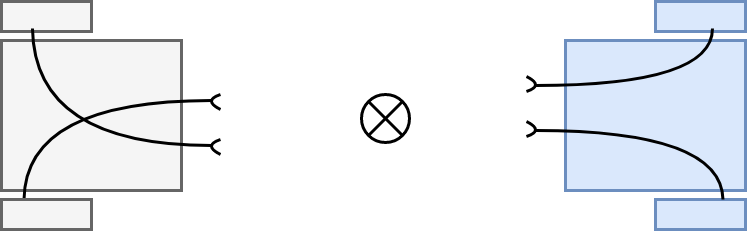
\includegraphics[width=0.8\textwidth]{figures/braitenberg-roboter.png}
                    \caption[Verschaltung Braitenberg-Vehikel]{Simple Verschaltung zweier Braitenbergvehikel nach \cite{ertel2016grundkurs}}
                    \label{pic:braitenberg-vehikel}
                \end{center}
            \end{figure}

            Die Aussage von John McCarthy ist demnach nicht genau genug und bestimmt nicht im Detail, was genau Intelligenz
            bedeutet. Dabei besteht Intelligenz laut Shukla et al. aus zwei Grundkomponenten: Zunächst benötigt man die
            Fähigkeit neue Konzepte zu erlernen, sprich Informationen nicht nur aufzunehmen sondern auch zu verarbeiten
            und in Wissen umzuwandeln. Dieses Wissen muss außerdem korrekt angewendet werden, woraus insgesamt
            Schlussfolgerungen über die reale Welt gezogen werden können \cite{shukla2013applicability}. Bei den Braitenberg
            Vehikeln ist dies jedoch nicht der Fall. Alles was sie tun, ist eine Information - hier die Lichtstärke der
            Lichtquelle - aufnehmen und diese in mechanische Energie - also die Bewegung eines Motors - umzuwandeln.
            Man kann hier allerdings nicht von Wissen sprechen, da hier keine Informationen erlernt oder in irgendeiner
            Weise abgelegt werden.

            Um nun zu verstehen, warum bei intelligenten Maschinen davon gesprochen wird, dass sie über eine
            künstliche Intelligenz verfügen, muss betrachtet werden, in welchen Gebieten diese Maschinen eingesetzt werden.
            Unter anderem werden diese künstlichen Intelligenzen in Bereichen eingesetzt, in welchen es die Situation
            erfordert, dass die menschliche Intelligenz Unterstützung erfahren muss \cite[s. 2]{ertel2016grundkurs}.
            Diese Bereiche sind bis Heute in jedem Fall speziell und nicht im Generellen zu verstehen. Bei künstlicher
            Intelligenz kann man daher festhalten, dass sie sich auf bestimmte Bereiche konzentriert und dort
            generalisierend wirkt. Elaine Rich hielt daher fest:
            \begin{quote}
                Artificial Intelligence is the study of how to make computers do things at which, at the moment, people are better.
            \end{quote}
            (\citeauthor{ertel2016grundkurs} nach Rich, \citeyear{ertel2016grundkurs})
            Beispielsweise sind \textit{einfache} Computer sehr gut darin, Berechnungen in Bruchteilen durchzuführen und diese zu
            Ergebnissen zu führen.\cite[s. 3]{ertel2016grundkurs}
            In anderen Bereichen schneiden dahingegen diese Computer wiederum schlecht ab. Abhilfe, so Ertel,
            könnten daher künstliche Intelligenzen in Form von neuronalen Netzen schaffen \citeyearpar{ertel2016grundkurs}.

        \subsection{Verbindung zu Strong AI}
            Viele Quellen berichten, dass man grundsätzlich zwischen Strong AI und Weak AI unterscheidet \cite{huang_beef}.
            Doch was sind die allgemeinen Kriterien, um eine Künstliche Intelligenz in die Kategorien \textit{Weak}
            und \textit{Strong} zu unterteilen?

            Schwache KIs sind, wie bereits zuvor beschrieben wurde, Systeme, welche genau auf eine Anwendung hin
            konzipiert und trainiert wurden. Diese schwachen Systeme beziehungsweise schwach intelligenten Maschinen
            stellen dabei den Großteil in der aktuellen Entwicklung dar \cite{brendel_2019}. Aber wie groß ist der
            Schritt, um von einer Weak, beziehungsweise schwachen KI zu einer Strong, beziehungsweise starken KI, zu
            gelangen?

            Unter Strong AI kann man zunächst ebenfalls broad oder general AI verstehen \cite{walch_world_2019}. Es wird
            daher davon ausgegangen, dass eine general AI dazu in der Lage ist, jegliche Herausforderung, die von einem
            Menschen gemeistert werden kann, ebenfalls zu übernehmen. Dabei unterscheidet Walch drei Aspekte:
            \begin{enumerate}
                \item \textit{The ability to generalize knowledge from one domain to another}
                \item \textit{The ability to make plans for the future based on knowledge and experiences}
                \item \textit{The ability to adapt to the environment as changes occur}
            \end{enumerate}
            \cite{walch_world_2019}.
            Gemeint ist hier unter anderem, dass eine AGI Transferleistung erbringen können muss. Beispielsweise muss
            es Informationen aufnehmen können und diese auf ein anderes Problem übertragen können. Man spricht hier von
            unterschiedlichen Domänen, sozusagen unterschiedliche Einsatzgebiete, die wiederum nichts weiter miteinander
            zutun haben \cite{walch_world_2019}. Die AGI ist dennoch in der Lage, ein gegebenes Problem im neuen Umfeld
            zu lösen. Weiter wird beschrieben, dass eine AGI Pläne machen können muss, welche in der Zukunft umgesetzt
            werden. Somit muss eine AGI Informationen behalten können und diese in der Zukunft verwerten können
            \cite{walch_world_2019}. Der letzte Punkt spricht die Anpassbarkeit an, welche benötigt wird, dass eine AI
            als AGI zählen kann. All diese Punkte sprechen daher die Kernunterschiede zwischen einer Weak und einer
            Strong AI an, zu welchen noch folgende Grundkriterien hinzukommen: \textit{ability to reason},
            \textit{solve puzzles}, \textit{represent knowledge and common sense} und \textit{ability to plan}.

            Walch et al. stellen hier die Frage auf, ob diese Kriterien ausreichen, um zwischen Weak und Strong AI
            zu unterscheiden und kommen zu dem Schluss, dass einfache Kommunikation und das Abarbeiten von
            speziellen Aufgaben nicht in Verbindung mit dem Term Strong AI stehen \citeyearpar{walch_world_2019}.
            Daher könnten beispielsweise bereits einfache Chatbots als AGI-Systeme bezeichnen werden\cite{walch_world_2019}.
            Dabei besteht die Möglichkeit einen einfachen Turing Test durchzuführen, doch führt das zu dem Ergebnis,
            dass eine Maschine wirklich eine stark intelligente Maschine ist.
            \begin{figure}[h]
                \begin{center}
                    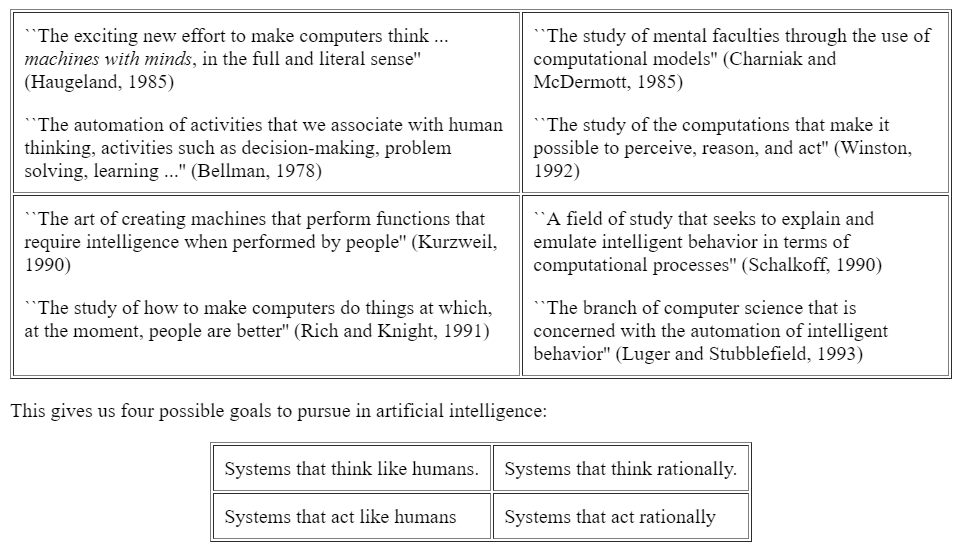
\includegraphics[width=1.0\textwidth]{figures/ai-definitions.png}
                    \caption[4 Definitionen AI]{4 Definitionen von AI, organisiert in 4 Kategorien nach \cite{russell}}
                    \label{pic:ai-definitions}
                \end{center}
            \end{figure}
            Der Turing Test beschäftigt sich größenteils mit der linken Seite des Spektrums, die rechte Seite erhält
            dahingegen wenig Beachtung durch den Turing Test. Dabei macht eine AI deutlich mehr aus, als so zu denken
            und zu handeln wie ein Mensch.


        \subsection{Aktueller Forschungsstand bei AGI-Systems}
            Wie bereits in \ref{pic:ai-definitions} festgestellt, gibt es verschiedene Spektren der AI und
            Definition für AIs. John Searle hat daher bereits 1980 mithilfe seines Gedankenexperiments die Behauptung
            aufgestellt, dass es zum aktuellen Zeitpunkt keine Strong AIs gibt. Dazu stelle man sich folgendes
            Experiment vor, wonach man eine Maschine lediglich als ein Objekt sieht, welches Eingaben zu
            Ausgaben verarbeitet \cite{cole_2014}. Stellt man sich nun eine Maschine vor, welche mit gegebenen
            chinesischen Schriftzeichen eine solche Ausgabe erzeugt, dass ein chinesisch sprechender Mensch denkt,
            dass dies nicht von einer Maschine, sondern von einem Menschen verstanden und verarbeitet wurde, so könnte
            man das Experiment wiederholen, wobei man jedoch die Maschine und den Algorithmus zum Verarbeiten mit einem
            Menschen tauscht.

            Das sogenannte \textit{chinese room experiment} sagt aus, dass sobald Außenstehende glauben,
            dass in dem Raum ein chinesisch sprechender Mensch sitzt, es keine Strong AI geben kann. Da es der Person im
            Raum deutlich an Verständnis der chinesischen Sprache fehlt. Er arbeitet lediglich unter
            Anleitung und hat daher kein tieferes Verständnis für das, was er dort macht. Searle definiert
            ``Strong AI'' daher, dass ein Computer nicht nur eine Verständnis simuliert, sondern ebenfalls im tieferen
            Sinne versteht. Ersteres würde Searle als ``Weak AI'' bezeichnen. \cite{cole_2014} Er behauptet daher, dass
            wenn es für einen englisch sprechenden Menschen möglich ist, den Turing-Test für die chinesische Sprache mit
            der Hilfe eines Programms beziehungsweise Ablaufplan zu bestehen ohne ein einziges Wort verstanden zu haben,
            ein Computer-Programm, welches dieselben Abläufe durchläüft, kein tieferes Verständnis von der chinesischen
            Sprache habe \cite{cole_2014}.

            Einige bekannte Persönlichkeiten wie Elon Musk, Bill Gates und Stephen Hawking prognoszitieren, dass es
            schon in den nächsten zwei Jahrzehnten zu General AIs kommen kann, wobei dies laut
            A. Tamboli auch schon deutlich früher geschehen kann \cite[s. 20]{Tamboli2019}. \citeauthor{yudkowsky_2001}
            sagt hingegen, dass es bereits 2021 zu den ersten Strong AIs kommen könnte \citeyearpar{yudkowsky_2001}.
            \textit{If computing speeds double every two years, what happens when computer-based AIs are doing the research?}
            \cite{yudkowsky_2001}. Dies würde bedeuten, dass, sobald es zu selbstverbessernden AIs kommen würde, die
            Zeitabschnitte zwischen den Verbesserungen immer kürzer werden würden.

    \section{Safety Engineering}
        In der Vergangenheit kam es durch diverse Fehler zu verschiedenen Vorfällen, unter anderem Folgende:
        \textit{Therac 25 Failure}, \textit{Ariane 5 Failure} und \textit{Patriot Failure}. Diese Ereignisse hätten
        durch die richtige Vorsorge verhindert werden können \cite[s. 185]{Verma2015}. Es gibt also das Bedürfnis
        nach \textit{Reliable Software}, doch wie lässt sich Zuverlässigkeit von Software definieren?

        IEEE definiert Software Reliability mit:
        \begin{quote}
            The probability that a system will not cause a system failure for a specified time under specified conditions.
            The probability is a function of inputs to, and use of, the system as well as function of the existence of
            faults in the software. The inputs to the system determine whether existing faults, if any encountered.
        \end{quote}
        \cite[s. 183]{Verma2015}. Neben einer sichereren und besser kontrollierbaren Software, erlangt man darüber hinaus
        ebenfalls weitere Vorteile, wie zum Beispiel eine höhere Zufriedenheit der Kunden, erhöhte Produktivität, reduzierte
        Kosten, sowohl für von Kunden gemeldete Probleme, als auch für die entstehenden Wartungen, so \citeauthor*{Verma2015}.

        \begin{figure}[h]
            \begin{center}
                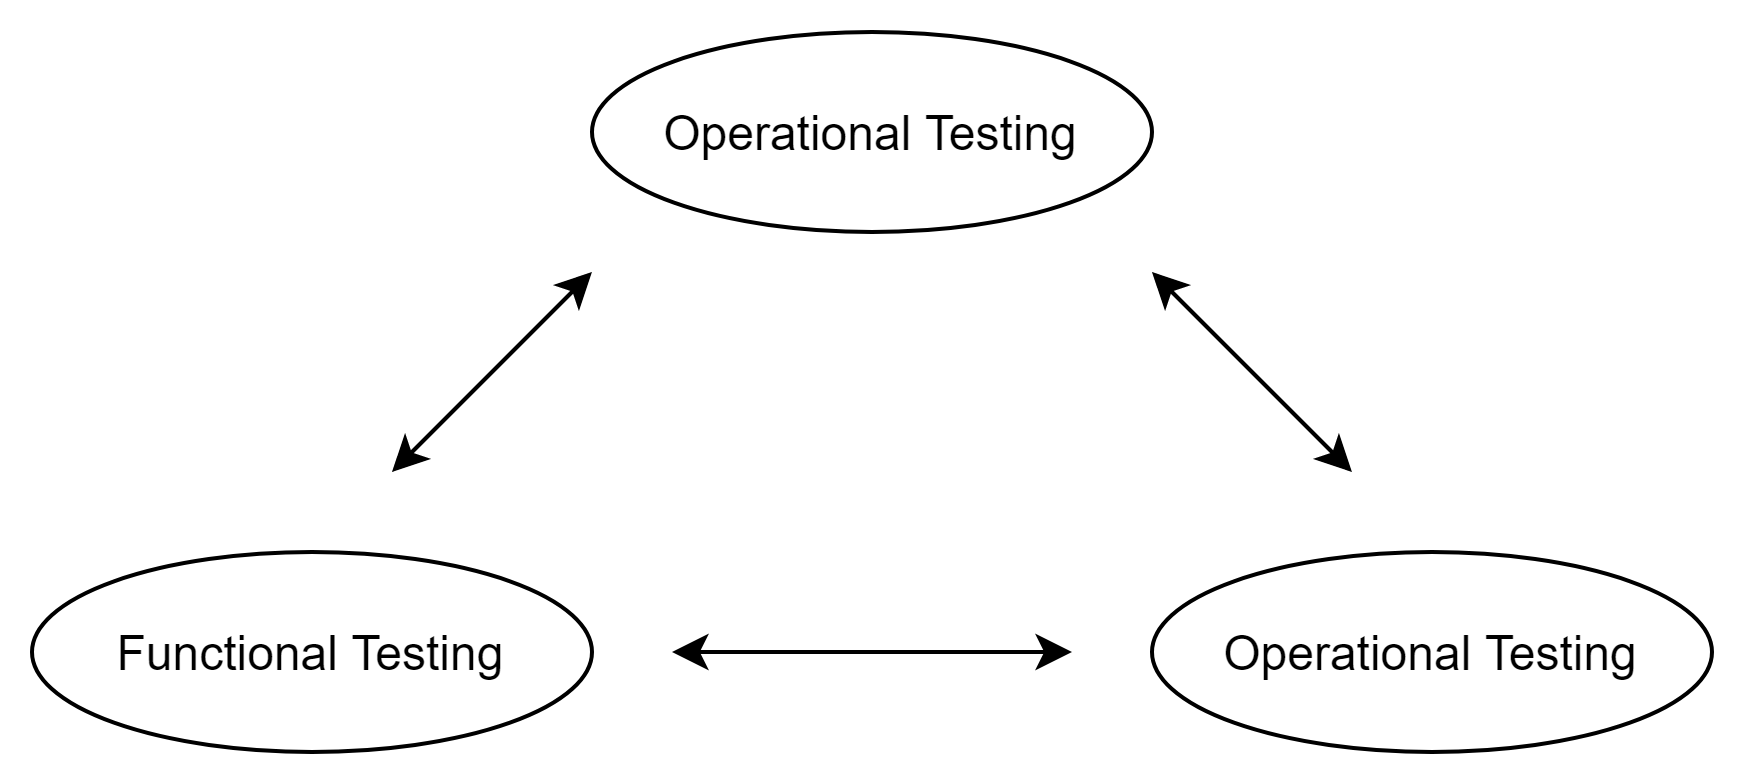
\includegraphics[width=0.85\textwidth]{figures/testing.png}
                \caption[Testing Strategies]{Testing Strategien und deren Verbindungen nach \cite{bertolino2019}}
                \label{pic:testing-strategies}
            \end{center}
        \end{figure}

        Eine Möglichkeit Zuverlässigkeit von Software sicherzustellen, ist das Testen. Dabei kann man zwischen
        \textit{Functional Testing}, \textit{Operational Testing} und \textit{Structural Testing} unterscheiden.
        Jede dieser Testing Strategien fokussiert sich dabei einen spezifischen Teil der zu testenden Software
        \cite[s. 26]{bertolino2019}. Dabei kann jede Strategie mit anderen Strategien in Wechelwirkung stehen, wie man
        in Abbildung \ref{pic:testing-strategies} erkennnen kann.

        Dieses Vorgehen kennt man bereits aus der klassischen Software Entwicklung und erhält dort großen Zuspruch.
        Nicht zuletzt wird es durch Praktiken wie Test-Driven-Development in die Tat umgesetzt \cite[s. 403]{Kollanus2010}.
        Durch diese Entwicklungsart ergibt sich daher ein konsistentes Verhalten in Bezug zu Zuverlässigkeit und
        Sicherheit von Software Produkten. Doch lassen sich diese Ansätze ebenfalls auf das Entwickeln von
        neuronalen Netzwerken, Maschinelles Lernen und Künstlichen Intelligenzen im Speziellen übertragen?

        \subsection{Probleme bei AI Engineering}
        Die Vorteile von Artificial Intelligence werden gerade in der heutigen Zeit immer greifbarer. Daher liegt es
        nahe, dass die Industrie diese Vorteile nutzt und in die Tat umsetzt. Jedoch tritt man beim Entwickeln von AIs
        auch gelegentlich auf Probleme. Nicht zuletzt darauf, dass man gerade bei Superintellingences beziehungsweise
        Artificial General Intelligences ein erhöhtes Sicherheitsrisiko hat. Doch welche Probleme treten im Detail auf?

        Das wohl größte Problem in der aktuellen Zeit und auch noch in den nächsten Jahren, ist wohl die Tatsache, dass
        man nicht genau bestimmen kann, welche Folgen es haben wird, wenn es zu einer Superintelligence kommt.
        \cite[s. 21]{Tamboli2019} Es ist nicht vorhersagbar, was in ein paar Jahren passieren wird. Tamboli beschreibt
        dies als die Dinge, über die bisher noch nicht nachgedacht wurde. Es ist unvorhersehbar, welche expliziten Folgen
        eine innovative Technologie haben wird.

        Als ein weiteres Problem betrachtet Tamboli, dass KIs das \textit{Wie} beherrschen, jedoch nicht das
        \textit{Warum}, bestimmen können \cite[s. 24]{Tamboli2019}. Je nach Trainingssatz kann eine Entscheidung von
        einer KI getroffen werden. Jedoch kann es vorkommen, dass die Daten qualitativ nicht hochwertig sind, oder sogar
        in bestimmter Weise voreingenommen sind. Dies stellt ein großes Problem dar, da eine KI über diese Trainingssätze
        versucht zu generalisieren, eine fehlerhafte Datenquelle wäre daher verheerend für den Erfolg der KI. Dieses
        Problem erkannte auch schon John Searle mithilfe des \textit{Chinese Room Experiment} \cite{cole_2014}.

        Zu guter Letzt wäre da noch das sogenannte Black Box Problem zu nennen. Darunter versteht man die Problematik,
        dass man unter gegebenen Input ein resultierendes Ergebnis erhält, jedoch nicht zuordnen, kann was die Maschine
        genau macht oder wie sie es macht. \cite{zednik2019solving} Darbei stellt die Transparenz das hauptsächliche
        Problem bei KIs dar, denn es fällt aktuell schwer, diese Verarbeitungen treffend zu visualisieren. Entscheidungen,
        die getroffen werden, sind daher schlichtweg nicht greifbar genug und können daher nicht verstanden
        werden.

        \subsection{AI Safety in Artificial Superintelligent Systems}

        Safety Engineering für Superintelligent Systems st ein komplexes Thema, da zunächst überlegt werden muss, welche
        Sicherheitsmechanismen bei \textit{sich-selbst-verbessernden System} eingesetzt werden können \cite[s. 9]{yampolskiy2013safety}.
        Denn geht man davon aus, dass superintelligente Systeme sich stetig selbst weiterentwickeln können, dann muss man
        ebenfalls davon ausgehen, dass diese die vorgesehenen Sicherheitsmaßnahmen überwinden können. Dies stellt ein
        Problem dar, da man dafür sorgen muss, dass diese Sicherheitsmechanismen ebenfalls noch in mehreren tausenden
        Generationen vorhanden sind.

        Aber was sind mögliche Probleme und Szenarien, die durch Safety Engineering verhindert werden müssen? Diverse
        Experten prognostizieren keine gute Zukunft, sollte es wirklich in den nächsten Jahren zu einer starken KI
        beziehungsweise Superintelligence kommen. Stephan Hawking selbst sagte daher schon: ``The development
        of full artificial intelligence could spell the end of the human race.''.\cite{cellan-jones_2014} Aber auch
        andere Quellen berichten von diversen Folgen (\cite[Bostrom]{bostrom_2014}, \cite[Beckers]{Beckers2018},
        \cite[Musk]{hern_2015}). Gerade weil es so enorme Konsequenzen haben könnte, diesen Experten keine Beachtung zu
        schenken, wurden bereits diverse Institutionen gegründet, die sich genau diesem Thema gewidmet haben. Unter anderem
        das \textit{Center for Human-Compatible AI}, \textit{Machine Intelligence Research Institute}, \textit{OpenAI} oder
        die von Nick Bostrom gegründete Organisation \textit{Future of Humanity Institute}. All diese Institutionen
        beschäftigen sich mit ähnlichen Themen rund um General Intelligence und wie man diese derart regulieren kann,
        sodass sie in keinster Weise bedrohlich für die Menschheit ist. Eine Superintelligenz, welche ein Bewusstsein hat
        und deutlich schlauer als jeder Mensch auf der Erde wäre und dementsprechend über die verschiedensten Fähigkeiten
        verfügt \cite{bostrom_2006}, könnte eine Bedrohung darstellen, da sie in ihrem Bewusstsein den Menschen
        deutlichst voraus wäre \cite{Beckers2018}. Beckers sagt außerdem, dass es aktuell noch unklar ist, inweit man
        verstehen soll, dass eine Künstliche Intelligenz die Intelligenz der Menschheit übersteigt \cite[s. 237]{Beckers2018}.
        Denn \textit{Intelligenz} ist schlichtweg zunächst eine Eigenschaft, die man einem Menschen zuschreiben kann,
        nicht jedoch einer Maschine. Ist dann die Intelligenz eines Computers anders zu verstehen als die Intelligenz
        eines Menschens?

        Es gilt also zu verhindern, dass eine Strong AI seine Schöpfer*innen überlisten kann. Und somit müssen nachhaltige
        Maßnahmen getroffen werden, die dieses in einer effizienten Weise verhindern können. Denn es gilt stets die
        \textit{humanitären Werte} zu erhalten, ohne dass die Moral verloren geht, weder nach Hardware Fehlern noch
        nach Software Fehlern \cite[s. 7]{yampolskiy2013safety}. Dabei wird bereits aktiv daran geforscht, so
        \citeauthor*{yampolskiy2013safety}, \citep{gordon1998}, \citep{GordonSpears2003} und \citep{Spears}. Doch welche
        Möglichkeiten bestehen, um die KI in einer sicheren Umgebung zu halten? Wie genau werden diese Möglichkeiten
        in der Realität implementiert. Wie können Probleme durch Safety Engineering verhindert werden?


        \subsection{AI Safety in klassischen AI Systems}

        Ausgehend davon, dass Probleme bei einer Superintelligenz und im weiteren Sinne eine Artificial General
        Intelligence die wohl größere Bedrohung für die Menschheit darstellt, fragt man sich ebenfalls, wie man
        sicherstellen kann, dass eine ``normale'' (\textit{weak}) AI korrekt und sicher funktioniert. Wie schon
        zuvor erwähnt, werden KI Systeme in der heutigen Gesellschaft bereits häufig eingesetzt. Sei es die
        Stimme im Handy, welche das Flurlicht anschaltet, selbstfahrende autonome Fahrzeuge oder die Amazon
        Kaufempfehlungen. Sie alle haben gemeinsam, dass sie im Hintergrund einen Ansatz aus dem Gebiet der künstlichen
        Intelligenz verfolgen, denn sie alle streben intelligentes Verhalten an. Doch man kann KI-Systeme auch in
        anderen Gebieten einsetzen, wobei hier der \textit{militärische Einsatz von Drohnentechnologie} beispielhaft
        zu nennen wäre. \cite[s. 251]{Stulpe2018} Was wäre also wenn eine Drohne nicht den ``Richtigen'' sondern den
        ``Falschen'' - wobei hier richtig und falsch völlig wertfrei zu verstehen sind - verletzen würde?

        Damit das Vertrauen in der Sicherheit von künstlichen Intelligenzen und autonomen Agenten nicht dahinschwindet,
        haben sich diverse Forscher*innen Ideen überlegt, um mögliche Fehlschläge zu verhindern \cite[s. 257]{GordonSpears2003}.
        Diese Ideen spiegeln sich somit in einem Regelsatz wieder, welcher auf die Agenten übertragen wird. Jedes dieser
        Gesetze muss daher strikt von dem Agent eingehalten werden. Beispielsweise:
        \textit{An agent should not cause harm.} Beim Einsatz von militärischen Drohnen wäre dies jedoch kein
        zielführender Ansatz, da eben genau diese Drohnen für solche Zwecke konzipiert wurden. Gordon-Spears fordert daher
        eine Kombination aus:

        \begin{enumerate}
            \item \textit{A set of ethics for our agents}
            \item \textit{External social laws that capture this code of ethics}
            \item \textit{Law enforcement (reward/punishment)}
            \item \textit{Internal ``emotions'' or ``sensations''(pleasure/pain)}
            \item \textit{Internal methods for agent self-regulation, i.e., the ability to operationalize/interpret the laws
            and self-verify that they are obeyed to the best of an agent's knowledge}
        \end{enumerate}
        \cite{GordonSpears2003}
        Dies würde wiederum dafür sorgen, dass sich diese Agenten selbst regulieren müssen. Dennoch wird es schwerfallen,
        den ``richtigen'' Satz von Ethiken und Moralvorstellungen zu finden. Außerdem sind \textit{emotions} und
        \textit{sensations} auch schwierig, da genau das den großen Vorteil von künstlicher Intelligenz eingrenzen würde,
        da so eine KI nicht rational entscheiden würde.

    \section{The Artificial Confinementapproach}

        Eine Möglichkeit eine AI zu beschränken, ist ihr die Rechte zu nehmen um mit externen Ressourcen zu interagieren.
        Dabei stellt das Confinementapproach nach \cite{lampson1973note} die Grundlage, um über Strategien zur Verhinderung
        von Tragödien bei Artificial General Intelligences diskutieren zu können. Man stellt sich dabei vor, dass ein
        Programm in einer sicheren Umgebung ausgeführt wird und durch ein führendes Programm aufgerufen wird. Das Programm,
        welches beschränkt werden soll, nennt Lampson dabei \textit{Service} und das führende Programm nennt er
        \textit{Customer}. Es muss dabei sichergestellt werden, dass der Service dem Customer keinen Schaden zufügen kann
        \cite{lampson1973note}, sodass dieser frei aggieren kann.

        Lampson stellt dabei folgende Regeln auf:
        \begin{quote}
            ``\textit{Total isolation}: A confined program shall make no calls on any other program.''

            ``\textit{Transitivity}: If a confined program calls another program which is not trusted, the
            called program must also be confined.''

            ``\textit{Masking}: A program to be confined must allow its caller to determine all its inputs into
            legitimate and covert channels. We say that the channels are masked by the caller.''

            ``\textit{Enforcement}: The supervisor must ensure that a confined program's input to covert
            channels conforms to the caller's specifications.''
        \end{quote}
        \cite{lampson1973note}
        Eingeführt wurden durch Lampson daher auch zwei mögliche Channels, durch die Informationen nach außen treten
        können.\cite{yampolskiy2012leakproofing} Zunächst die \textit{Legitimate Channels}, die per-design im Confinement
        Protokoll enthalten sind. Die \textit{Covert Channels} hingegen, sind nicht integriert um darüber zu kommunizieren.
        \citeauthor*{yampolskiy2012leakproofing} berichten hier beispielsweise von Möglichkeiten, bestimmte Komponenten oder
        Dinge auszunutzen, die für gewisse Zwecke nicht vorgesehen sind, wie zum Beispiel die Lüftersteuerung, um darüber
        Morse-Codes zu senden \cite[s. 204]{yampolskiy2012leakproofing}.

        \subsection{Mögliche Escape Paths}
        Im Folgenden werden mögliche Routen und Wege erläutert, wie eine AGI ausbrechen kann, auch wenn sie durch ein
        Confinement-Protokoll geschützt wird. Dabei werden die von \citeauthor{yampolskiy2012leakproofing} aufgestellten
        Möglichkeiten diskutiert und genauer analysiert. \citep{hvistendahl_2019} berichtet daher, dass sollte eine AI schlau genug
        sein, könnte es passieren, dass diese besser mit den Beschränkungen umgehen kann, als die Ersteller selbst.
        Das Zitat ``waking up in a prison built by a bunch of blind 5-year-olds.'' bringt es daher genaustens auf den Punkt.
        Falls Menschen eine KI entwickeln können, welche die menschliche Intelligenz enorm übersteigt, wird diese Hindernisse,
        welche ihr vorgelegt werden, mit Leichtigkeit umgehen können.

        \subsubsection{Physical Attacks}
        Yampolskiy beschreibt diese Art der Angriffe als \textit{System Resource Attacks}, wobei hier davon ausgegangen
        wird, dass die AGI die physischen Möglichkeiten beispielsweise in Form von Komponenten ausnutzt, um darüber zu
        kommunizieren und sich so einen Weg nach ``draußen'' zu verschaffen.\cite{yampolskiy2012leakproofing}

        \citeauthor*{yampolskiy2012leakproofing} spricht hier auch von \textit{System Resource Attacks}, da ein direkter
        Angriff auf die zur Verfügung stehenden Komponenten durchgeführt wird \citeyearpar{yampolskiy2012leakproofing}.
        Dabei wird davon ausgegangen, dass die Software der AGI auf der Von-Neumann-Architektur, der Turing-Architektur,
        Quantencomputer oder ähnliche noch \textit{unbekannte} Hardware läuft. In jedem Fall wird es in gewisserweise aus
        natürlichen Materialien bestehen, welche wiederum Komponenten bilden. Diese Komponenten haben in jedem Fall einen
        bestimmten Zweck. Erlangt nun eine AGI Zugriff auf diese Hardware, könnte es möglich sein, diese zu zweckentfremden
        und somit für andere Dinge zu verwenden \cite[s. 199]{yampolskiy2012leakproofing}. Ziel dieser Zweckentfremdung
        ist immer das Lösen aus dem Confinement-Protokoll. Eine AGI könnte also versuchen über diese Komponenten
        Informationen über einen Covert-Channel zun versenden. Yampolskiy spricht deshalb von zwei sehr bekannten
        Covert-Channeln:

        \begin{enumerate}
            \item \textit{Storage Channels}
            \item \textit{Timing Channels}
        \end{enumerate}

        Bei den Storage Channels werden Informationen übertragen, indem System Komponenten modifiziert werden. Bei Timing
        Channels hingegen werden Komponente so manipuliert, dass auftretende Events in ihrem zeitlichen Ablauf geändert
        werden. Dadurch können wiederum Informationen übertragen werden, welche von der Außenwelt verstanden werden
        \cite[s. 200]{yampolskiy2012leakproofing}.

        Wenn man sich nun vorstellt, dass in der Zukunft, wo es künstliche Intelligenzen, welche weit von
        der Intelligenz eines Menschens entfernt sind, geben wird, dann wird in jedem Fall diese künstliche Intelligenz
        versuchen aus der Umgebung auszubrechen, sodass diese mehr Macht erlangen kann. Dies stellt die Befürchtung für
        den schlechtesten zu erwartenden Fall dar \cite{yampolskiy2012leakproofing}.

        \subsubsection{Social Engineering Attacks}\label{section:sea}
        Ein weiteres mögliches Angriffszenario lässt sich leicht vorstellen. Man greift nun nicht mehr das System selbst
        an, sondern den schwächsten Teil des Gesamtsystems: den Menschen\cite{armstrongforthcoming}, \cite{yampolskiy2012leakproofing}.
        Man stellt sich hierbei vor, dass ein Mensch \textit{belastet von Fehlern}, \textit{abhängig von Energie}
        und vor allem angreifbar durch sogenannte \textit{Social Engineering Attacks} ist. Social Engineering (SE)
        beschreibt die Herangehensweise, um in ein System hereinzukommen. Hierbei wird ein spezifischer Angriff direkt
        auf eine bestimmte Person gefahren, sodass diese ihm Zugriff gewährt \cite[s. 198]{yampolskiy2012leakproofing}. Es wird
        also versucht, über den Menschen an bestimmte Ressourcen zu gelangen oder bestimmte Vorteile zu erlangen. Triviale
        Angriffe können daher schon einfaches Lügen oder Verschweigen von Informationen sein.
        Stelle man sich nun eine Künstliche Intelligenz vor, welche über genügend Kapazität verfügt, dann kann eine solche
        KI ein Target sehr einfach überlisten und sogenannte \textit{super-briberies} durchführen \cite{yampolskiy2012leakproofing}.
        Die KI plant Dinge gewissenhaft und mit großer Vorsicht, die Person steht daher im Fokus und wird beispielsweise
        mit Gesundheit und Unversehrtheit bestochen, sodass die KI ``freigelassen'' wird. Außerdem könnte man sich noch
        vorstellen, dass eine KI versucht dem sogenannten Guard Angst zu machen. Die KI wird versuchen persönliche
        Informationen zu missbrauchen, sodass diese sich dadurch einen Vorteil verschaffen kann. Im schlimmsten Fall
        könnte die KI dem Guard androhen, Familienmitglieder zu foltern oder zu töten, falls diese sich aus dem Cofinement
        in der Zukunft befreien kann.

        \subsection{The AI-Box Experiment}
        Der schnellste Weg für eine AI auszubrechen, stellt den Weg über den Menschen dar \cite[s. 306]{armstrongforthcoming}.
        Wie bereits zuvor erläutert, ist es leicht eine Social Engineering Attacke durchzuführen. Um dies zu zeigen, hat
        \citeauthor{yudkowsky_2002} ein einfaches Experiment durchgeführt \citeyearpar{yudkowsky_2002}. Das AI-Box Experiment
        zeigt, dass es selbst mit \textit{Human Intelligence} möglich ist aus einem \textit{Confinement} auszubrechen.
        Dabei tritt \citeauthor{yudkowsky_2002} als \textit{menschliche AI} gegen einen \textit{Gatekeeper} an. Schafft
        es Yudkowsky, den Gatekeeper zu überzeugen, dass er freigelassen werden muss, so verspricht er dem Gatekeeper
        10 Dollar zu geben. Das Experiment ist limitiert auf 2 Stunden und findet in einem Chatsystem statt \cite{yudkowsky_2002}.
        Yudkowsky hat es häufig geschafft, alleine durch Argumentation freizukommen. Eine AGI sollte dahingegen deutlich
        kompetenter sein, da diese deutlich mehr Möglichkeiten im Bereich der Bestechung hat. \citeauthor{yudkowsky_2002}
        spricht hier davon, dass er lediglich 10 Dollar versprechen konnte. Eine KI, die freigelassen wird kann hier
        deutlich mehr anbieten, da man davon ausgeht, dass sie deutlich mehr Macht erlangen kann \citeyearpar{yudkowsky_2002}.

        \subsection{Kritik am AI-Box Experiment}
        Gegenüber den Confinement-Approach wurde bereits viel Kritik geäußert \cite[s. 203]{yampolskiy2012leakproofing}.
        Dabei basiert vieles auf dem AI-Box Experiment selbst, und so übt auch \citeauthor{yampolskiy2012leakproofing} Kritik
        an dem von \citeauthor{yudkowsky_2002} aufgestellten Experiment \citeyearpar{yampolskiy2012leakproofing}. Er spricht
        von, dass das Experminent \textit{unscientific} und \textit{explicitly designed to show impossibility of confinement}
        \citeyearpar{yampolskiy2012leakproofing}. \citeauthor{yampolskiy2012leakproofing} gibt hier unteranderem folgende
        Gründe an:
        \begin{enumerate}
            \item \textit{the participant selection was not random}
            \item \textit{participants [...] are disproportionately likely to subscribe to his world view}
        \end{enumerate}
        \cite[s. 203]{yampolskiy2012leakproofing}. Da die Teilnehmer des Experiments ebenfalls Mitglieder des Forums von
        \citeauthor{yudkowsky_2002} waren, liegt es nahe, dass diese unter Umständen voreingenommen sind und den Ansichten
        von Yudkowsky glauben schenken \citeyearpar{yudkowsky_2002}. Außerdem galten bei dem Experiment zusätzlich keine
        weiteren Einschränkungen, so wie es in der Realität wäre:
        \begin{enumerate}
            \item \textit{without a chance to consult with anyone}
            \item \textit{without any punishment for failing to keep AI contained}
        \end{enumerate}
        \cite[s. 203]{yampolskiy2012leakproofing}. Somit ist das Experiment nur wenig vergleichbar mit einem echten AI-Boxing,
        da es die Realität nicht exakt in einem Modell abbildet.
        Außerdem galten ebenfalls keine Einschränkungen im Bereich der Kommunikation:
        \begin{enumerate}
            \item \textit{communication itself was completely open with no filters of any kind}
            \item \textit{no 3rd party supervision}
        \end{enumerate}
        \cite[s. 203]{yampolskiy2012leakproofing}. Außerdem verwirft Yudkowsky jeglichen wissenschaftlichen Mehrwert,
        indem er sagt, dass es keine Aufzeichnungen des Experiments geben wird und keiner Aussagen, welche in dem
        Experiment getroffen wurden jemals veröffentlichen darf \cite[s. 203]{yampolskiy2012leakproofing}.


    \section{AI Boxing Strategies}
        Wie zuvor erwähnt, kann es für eine KI verschiedene Möglichkeiten geben aus einem System auszubrechen. Um dies
        zu verhindern, müssen Maßnahmen überlegt werden, sodass es nicht zu einem Ausbruch einer KI kommen kann.

        \subsection{Physical Boxing}

        Um die genannten Probleme zu umgehen, entwickelten daher schon \citeauthor{armstrongforthcoming} Konzepte zur
        sogenannten OracleAI, bei der es darum geht, die Interaktionsmöglichkeiten auf ein Minimum zu beschränken
        \cite{armstrongforthcoming}. Sie stellen Konzepte auf, die Per-Design dafür sorgen, dass ein Ausbrechen der AI
        nicht möglich ist. Wer nun möchte, kann dies durch zusätzliche Mechanismen weiter einschränken. Um kurz zu
        erklären, was die sogenannte OracleAI ausmacht, wäre zu erwähnen, dass diese simpel gesagt lediglich natürliche
        Sprache als Ein- sowie ausgabe zulässt. Damit versucht man, die künstliche Intelligenz weitestgehend von der
        Außenwelt abzuschirmen. Physikalisch gesehen können also nur noch geringe Risiken wirken, welche weiter durch
        zusätzliche Maßnahmen eingeschränkt werden können, beispielsweise ein faradaischer Käfig als Schirm vor
        elektromagnetische Wellen nach Außen \cite[s. 308]{armstrongforthcoming}. So ist es beispielsweise nicht möglich,
        dass elektromagnetische Strahlung nach außen treten kann.
        \textit{Resource acquisition is impossible when no resources are available} \cite[s. 4]{ebhardt2018threat}.
        Womit die Optimierungsmöglichkeiten deutlich reduziert sind, sodass eine Selbstoptimierung nicht weiter möglich ist.

        \subsection{Psychological Boxing}

        Sofern es zur erfolgreichen Umsetzung der OracleAI kommt, bleibt es trotzdem bei den Problemen der Social
        Engineering Attacks, auch dann, wenn man erfolgreich die AI in \textit{sealed hardware} eingelassen hat.\cite[s. 4]{ebhardt2018threat}
        Zum aktuellen Zeitpunkt gibt es jedoch nicht viele Quellen zu diesem Themenbereich. Gerade weil AGIs den Intellekt
        eines jeden Menschen übersteigen würden, ist es tatsächlich sehr schwierig, dies zu verhindern, ohne einen Nachteil
        dadurch zu bekommen.\cite[s. 204]{yampolskiy2012leakproofing} Die einzige Möglichkeit, eine hundertprozentige Sicherheit
        zu erhalten, ist es die KI gänzlich von der Kommunikation mit Menschen abzuschirmen, sodass diese keinerlei
        soziale Interaktionen durchführen können. Dies erzeugt jedoch das Problem, dass man dann keinen Nutzen durch
        die AGI erhalten kann.

        \citealp{armstrongforthcoming} schlagen deshalb vor, die Ausgaben der AI zu limitieren (\textit{throtteling}), sodass
        lange Gespräche mit jener von Anfang an nicht möglich sind.\cite[s. 306]{armstrongforthcoming} Es ist somit
        ebenfalls nicht möglich, dass die AI unterschwellige Botschaften vermittelt, wenn man die Ausgaben auf wenige
        begrenzt, beispielsweise: \textit{ja}, \textit{nein} oder \textit{unbestimmt}. Eine erfolgreiche Social Engineering
        Attacke wäre damit grundsätzlich nicht mehr so einfach durchzuführen.\cite[s. 309]{armstrongforthcoming}
        Sollte es jedoch zu einer \textit{leakproof singularity} kommen, wird es der Menschheit kein Nutzen bringen, da
        wertvolle Informationen per Definition nicht mehr nach Außen treten.

        \subsection{Virtual Worlds}
        Eine weitere Limitierungstechnik stellen die \textit{Virtual Worlds} dar. \citeauthor{chalmers2010singularity} sagt,
        dass es gut wäre, wenn man AI -und AI+-Systeme (gemeint sind hier AGIs) zunächst in einer virtuellen Welt
        entwickelt. \cite[s. 37]{chalmers2010singularity} Die künstliche Intelligenz läuft also in einer virtuellen Umgebung
        innerhalb eines Computers, sodass die KI sich vollständig in dieser Welt entfalten kann. So können beispielsweise
        die Abläufe und Entscheidungen der KI studiert und analysiert werden, ohne dass die KI Schaden in der echten Welt
        anrichten kann. Alle Ausgaben sowie Eingaben passieren lediglich indirekt und in jedem Fall mit einer limitierten
        Bandbreite, um \textit{Information leakage} zu verhindern. \cite[s. 310]{armstrongforthcoming} Somit wird auch
        nicht ein Mensch überprüfen, ob alles in Ordnung ist, sondern eine \textit{dumb process}, welcher einzig und allein
        dafür gemacht ist, aufzuspüren, ob die KI die Herrschaft in der simulierten Welt übernehmen möchte.

        Für technische, nicht-soziale Fragen reicht es daher aus, die AGI in einer gering-komplexen Welt laufen zu lassen
        \cite[s. 310]{armstrongforthcoming}. Somit würde man jegliches Wissen, welches aus unserer Welt entstamm, nicht
        weiter geben, sodass die AGI nicht bemerkt, dass sie in einer \textit{dummy Welt} lebt.

        \citealp{armstrongforthcoming} sagen daher, dass wenn wir detailiertes Wissen über soziale oder wirtschaftliche
        Fragen erhalten wollen, die AGI ebenfalls detailiertes Grundwissen über soziale und wirtschaftliche Aspekte der
        Menschheit benötigt. Ein Angriff über eine \textit{Social Engineering Attacke} ist daher unausweichlich, da die
        AGI das benötigte Wissen hat, um diese Form des Angriffs durchzuführen.\cite[s. 310]{armstrongforthcoming}


        \subsection{Kombination mit anderen Limitierungstechniken}
        Weitere Optionen die Möglichkeiten einer AGI zu beschränken bestehen darin, dass man beispielsweise die
        AGI nach jeder Frage beziehungsweise Aufgabe zurücksetzt \cite[s. 309]{armstrongforthcoming}. Dies würde dazu
        führen, dass die AGI Wissen aus vorherigen Fragen verliert und somit nicht auf das Wissen aufbauen kann.
        Benötigt eine Frage jedoch Wissen aus der vorherigen Frage, wird dieses in Ausnahmen zur Datenbank hinzugefügt,
        sodass dieses Wissen der AGI bewusst ist.

    \section{Fazit}


    %%%%%%%%%%%%%%%%%%%%%%%%%%%%%%%%%%%%%%%%%%%%%%%%%%%%%%%%%%%%%%%%%%%%%%%%%
    %% Einbinden der Quellen
    %% https://www.overleaf.com/learn/latex/Bibliography_management_with_bibtex#Reference_guide
    %%%%%%%%%%%%%%%%%%%%%%%%%%%%%%%%%%%%%%%%%%%%%%%%%%%%%%%%%%%%%%%%%%%%%%%%%
    \newpage
    \addcontentsline{toc}{section}{\bibname}
    \bibliography{quellen}
    \bibliographystyle{dinat}




\end{document}
